\section{Lecture 8: Relating Unit Step and Unit Impulse}


\subsection{Impulse Response of for an RC circuit}
In the discussion about the importance of abstraction, we had come across two systems, the RC circuit, and the mass-force system, which had the same behaviour. Now, since the RC circuit system is a Linear Shift-Invariant system, it would be useful to acquire its unit impulse response, since this will empower us to obtain the output signal, for any given input signal.\\
\indent Recall that for the RC circuit system, we took the voltage applied across the resistor and the capacitor to be the input voltage ($V_{in}$ - the input signal), while the voltage across the capacitor to be the output voltage ($V_C$ - the output signal). (fig. 1)
\begin{figure}[H]
	\centering
	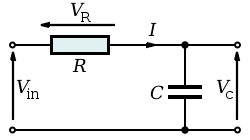
\includegraphics[width=0.4\textwidth]{./rc.png}
	\caption{RC circuit diagram}
\end{figure}
\indent Now, we had defined the unit impulse as a limiting case of the $\delta_\Delta$ function, whose width was $\Delta$, and whose area under the curve was unity.\\
\indent To find the unit impulse response, we need to go back to the differential equation governing the RC circuit. We know that the current in the circuit is proportional to the derivative of the capacitor voltage. i.e.
$$I=C\frac{dV_C}{dt}$$
\indent On integrating both the sides w.r.t. t, we get 
$$\int I dt = CV_C$$
\indent Instead of dealing with the Voltage directly, we will look at the integrated form. Thus arises the question: What is the integral of the unit impulse?
\subsubsection{Integral of the unit impulse}
Consider the $\delta_\Delta$ function centred at $t_0$. Now consider the running integral:
$$\textrm{Running Integral of }\delta_{\Delta,t_0} = \int_{-\infty}^t \delta_{\Delta,t_0}(\lambda)d\lambda$$
\indent Let us now divide the $\delta_{\Delta,t_0}$ function into three regions(fig. 2(a)):
\begin{itemize}
\item Region 1: The region $t<t_0$
\item Region 2: The region where $t_0< t <t_0+\Delta$
\item Region 3: The region $t>t_0+\Delta$
\end{itemize}
\indent We can see that the integral in Region 1 is zero since $\delta_{\Delta,t_0}$ is $0$ and that the only region where we need to calculate the integral is Region 2.\\
\indent The integral of a constant function is a linear function, and since we know that the area under the $\delta_\Delta$ function is unity, it is clear that the running integral increases linearly from 0 at $t=t_0$ to 1 at $t=t_0+\Delta$ after which, it remains 1 in Region 3. (fig. 2(b))
\begin{figure}[H]
        \centering
        \begin{subfigure}[b]{0.5\textwidth}
                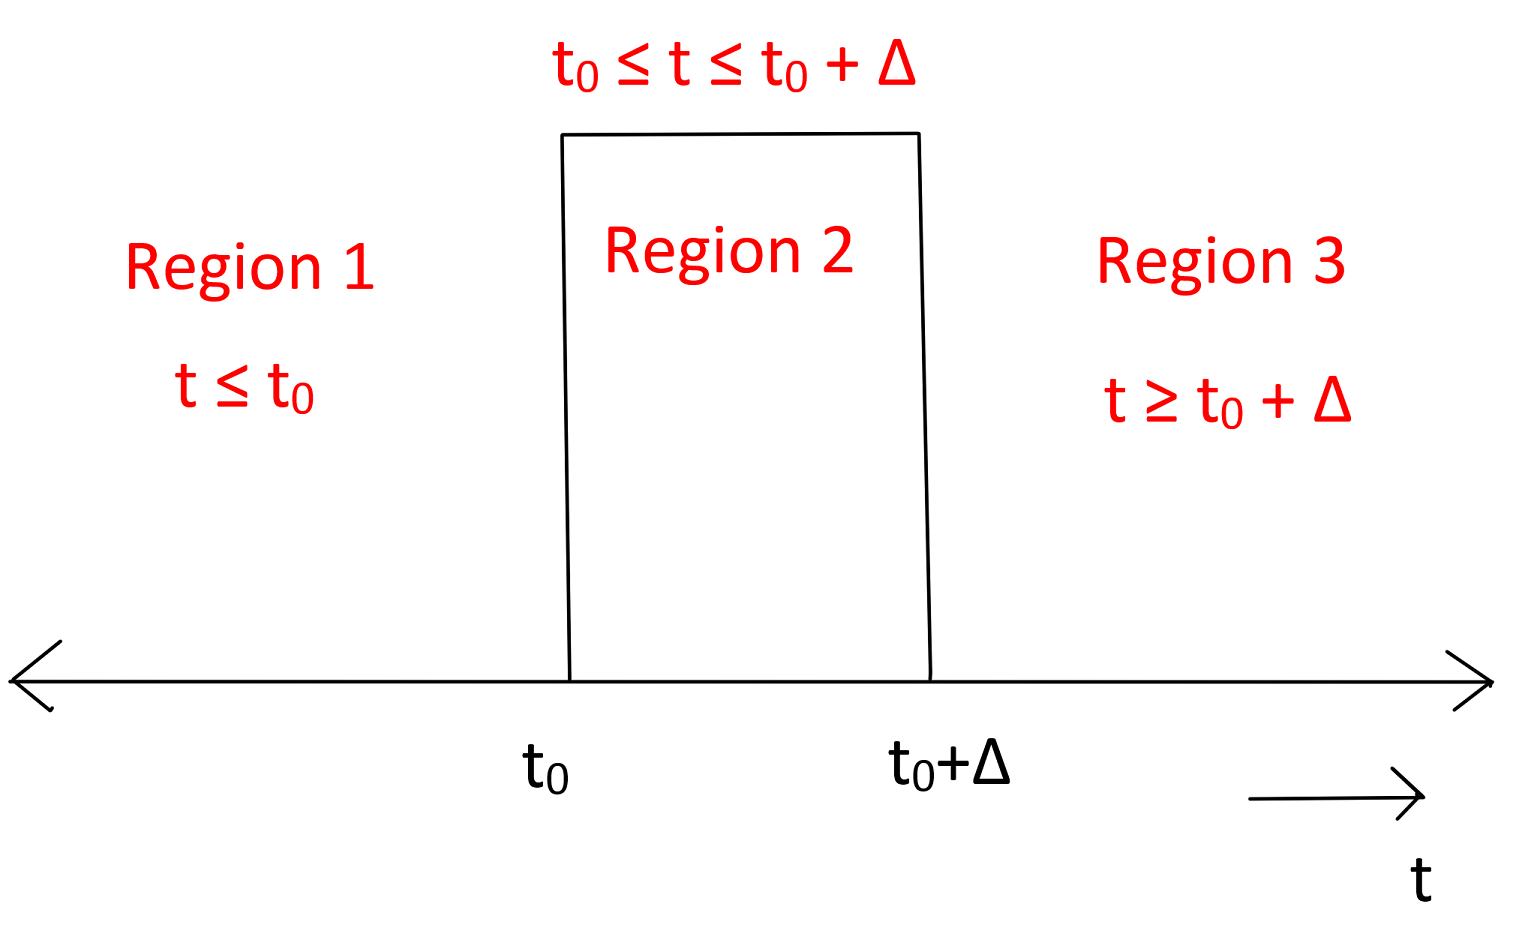
\includegraphics[width=\textwidth]{./regions_of_delta.png}
                \caption{Dividing the $\delta_\Delta$ function into 3 regions}
        \end{subfigure}
        \quad
	~	\quad
        \begin{subfigure}[b]{0.5\textwidth}
                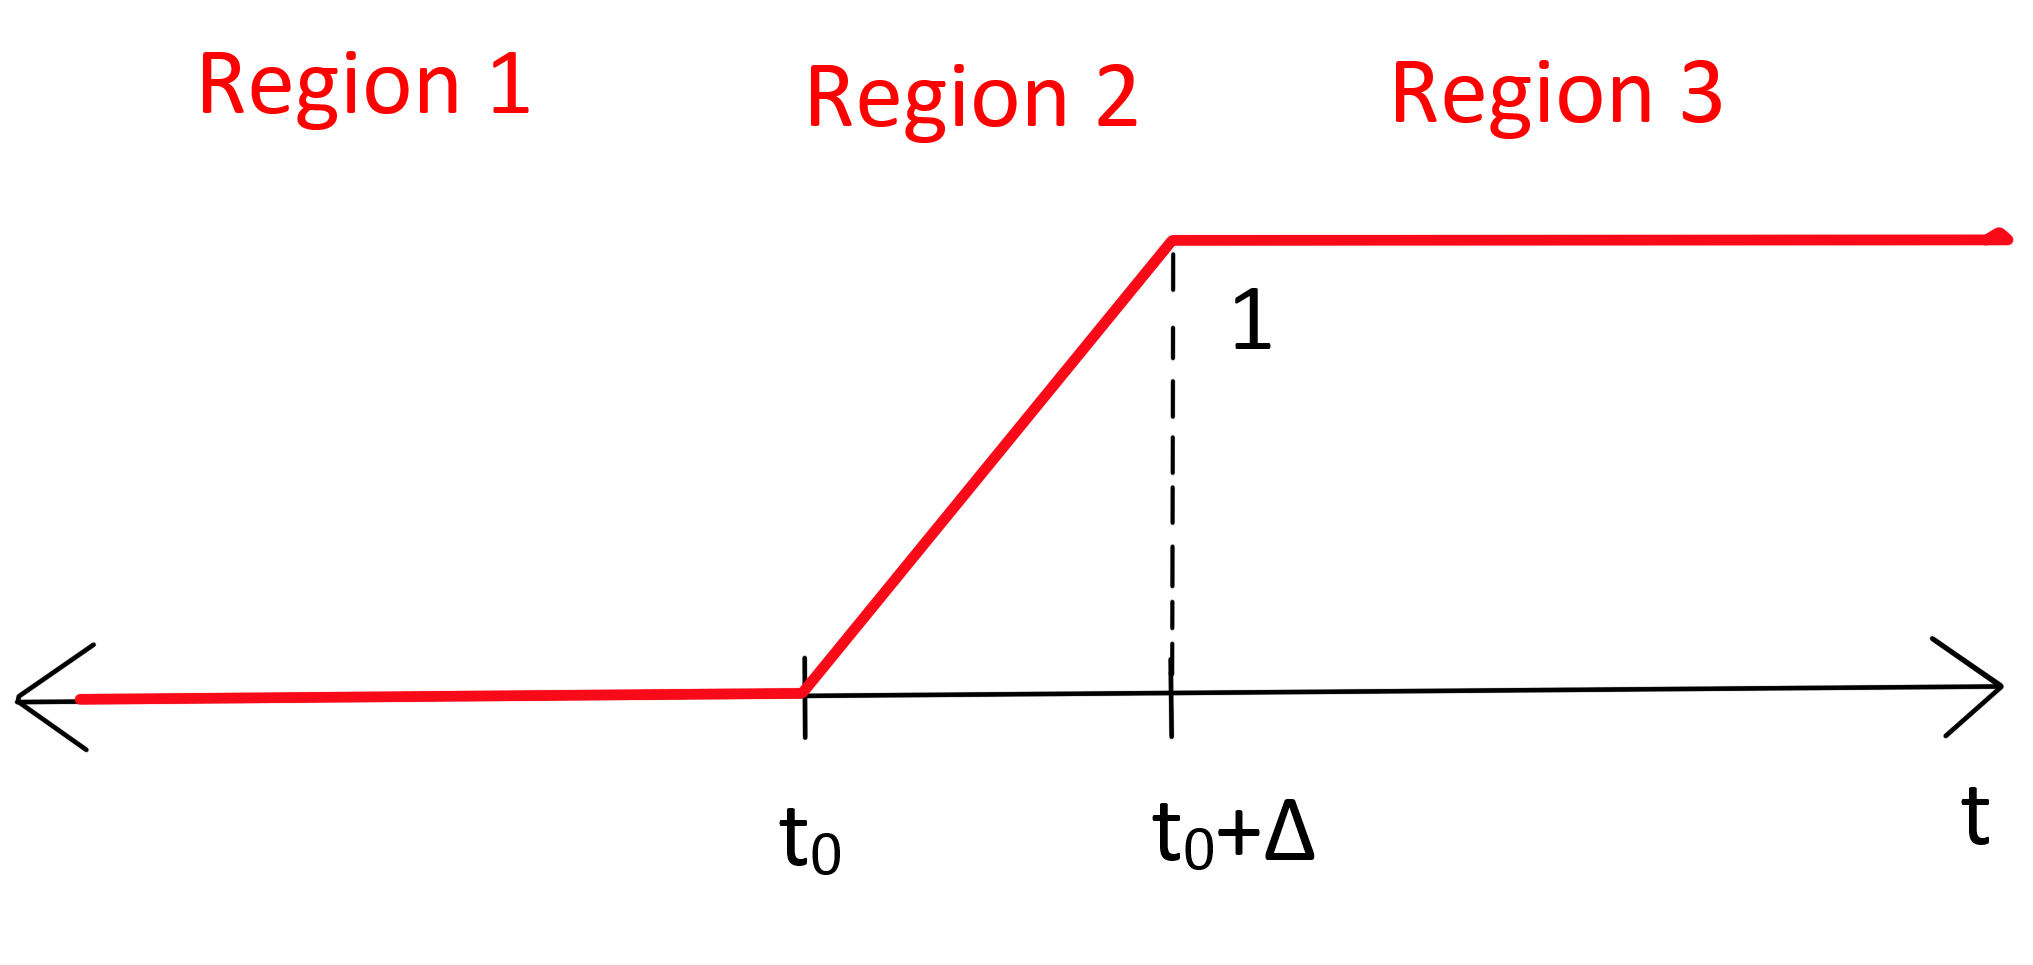
\includegraphics[width=\textwidth]{./running_integral_of_delta.png}
                \caption{Running integral of delta function}
        \end{subfigure}
        \caption{}
\end{figure}
\indent Now, to find the unit impulse response, we need to let $\Delta\rightarrow 0$. Clearly, Region 2 vanishes and we get the unit step, located at $t_0$.
Thus, 
\\\\
\noindent\fbox{%
    \parbox{\textwidth}{%
       \textbf{The running integral of the unit impulse is the unit step function, and the derivative of the unit step function is the unit impulse}
    }%
}\footnote{Note that in the classical sense of the derivative, it is not possible to take the derivative of the unit step at the origin, since it is a discontinuous function. Just as the unit impulse is not really a function, but a generalized function, the derivative of the unit step function is not a usual derivative, but is a `generalized derivative'. However, without going in the subtleties of the definition of a generalized derivative, we shall move ahead without distinguishing between the classical and generalized derivatives}
 
$$\textrm{Unit Impulse}\xrightarrow {\textrm{running integral}} \textrm{Unit Step}$$
$$\textrm{Unit Impulse}\xleftarrow {\textrm{derivative}} \textrm{Unit Step}$$
\indent Now, the derivative of a function $x(t)$ is defined as:
$$\frac{dx(t)}{dt}=\lim_{\Delta\rightarrow 0}\frac{x(t+\Delta)-x(t)}{\Delta}$$
\indent	The term $x(t+\Delta)$ can be considered as the function $x(t)$ shifted to the left by $\Delta$ units. Thus, the derivative can be thought of as the difference of the original function and a shifted version of the same function, divided by the shift in the limit of the shift going to zero. This is a more `Signals and Systems' way of thinking of derivatives of signals. The original aim of this exercise was to find the unit impulse response of the RC circuit. But instead of finding the unit impulse response, let us first find the unit step response. It can be shown that the expression for the unit step response will be $$(1-e^{-\frac{t}{\tau}})u(t)$$
where, $\tau=RC$ and $u(t)$ is the unit step function. This can be derived using knowledge of differential equations and can be verified by substituting in the RC circuit equation. Physically, we can argue that the the potential across the capacitor (i.e.the output voltage) cannot rise suddenly, and thus increases gradually and asymptotically towards a maximum value, for $t>0$.\\
\indent Now let us come back to the derivative of the unit step function. If we denote the unit step function by $u(t)$, its derivative will be:
$$\frac{du(t)}{dt}=\lim _{\Delta\rightarrow0}\frac{u(t+\Delta)-u(t)}{\Delta}$$
This is the difference between $u(t)$ and its shifted version, dicided by $\Delta$ (fig. 3(a))
\begin{figure}[H]
	\centering
	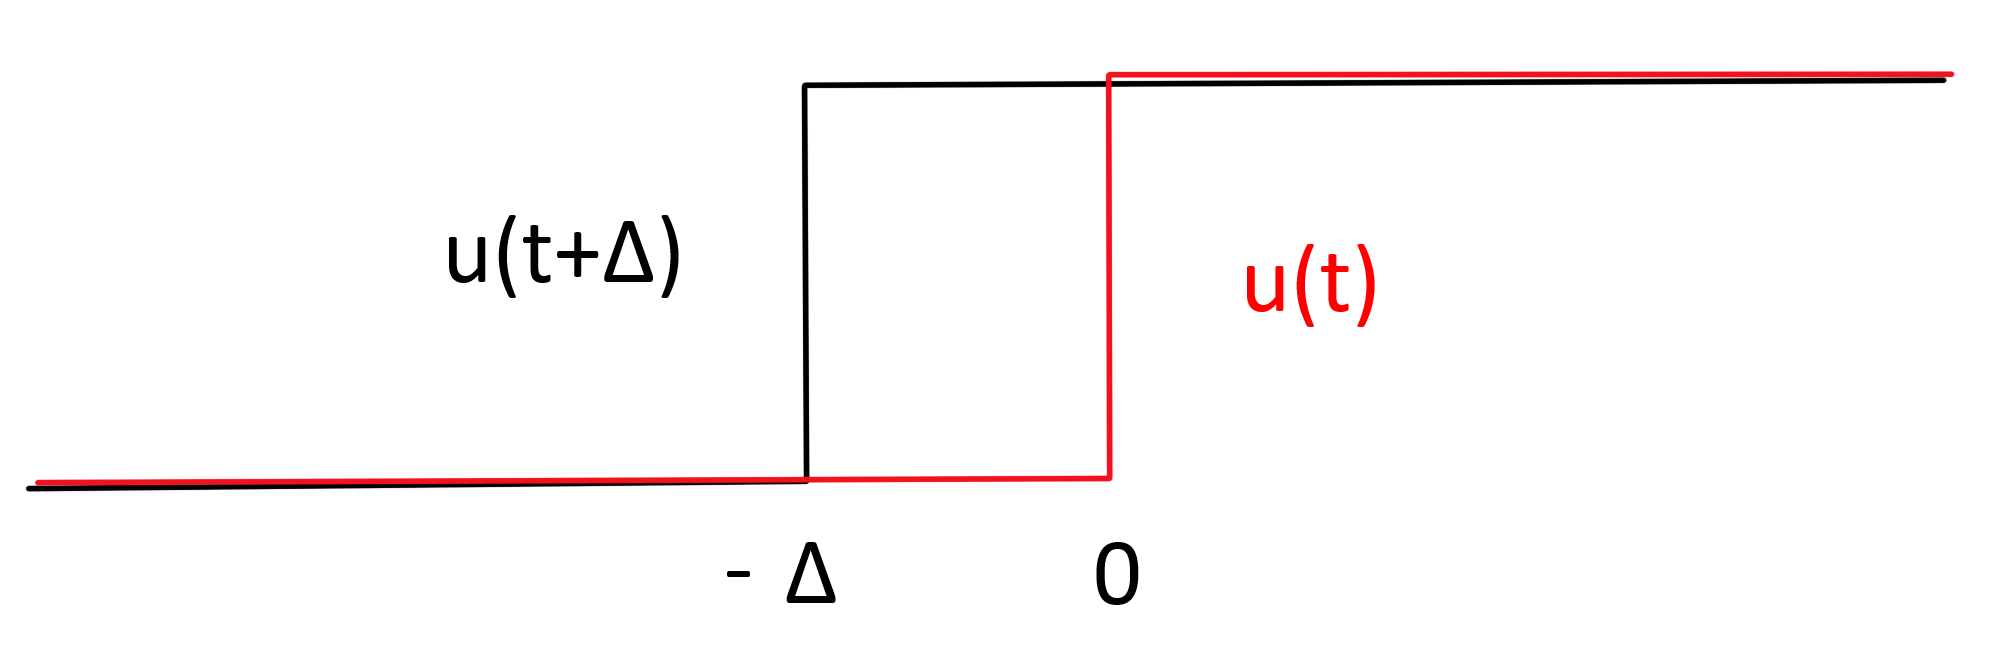
\includegraphics[width=0.6\textwidth]{./difference_deltas1.png}
	\caption{$u(t)$ and $u(t+\Delta)$}
\end{figure}
\indent	Now, talking their difference and dividing by $\Delta$ (fig. 3(b)), we get: 
\begin{figure}[H]
	\centering
	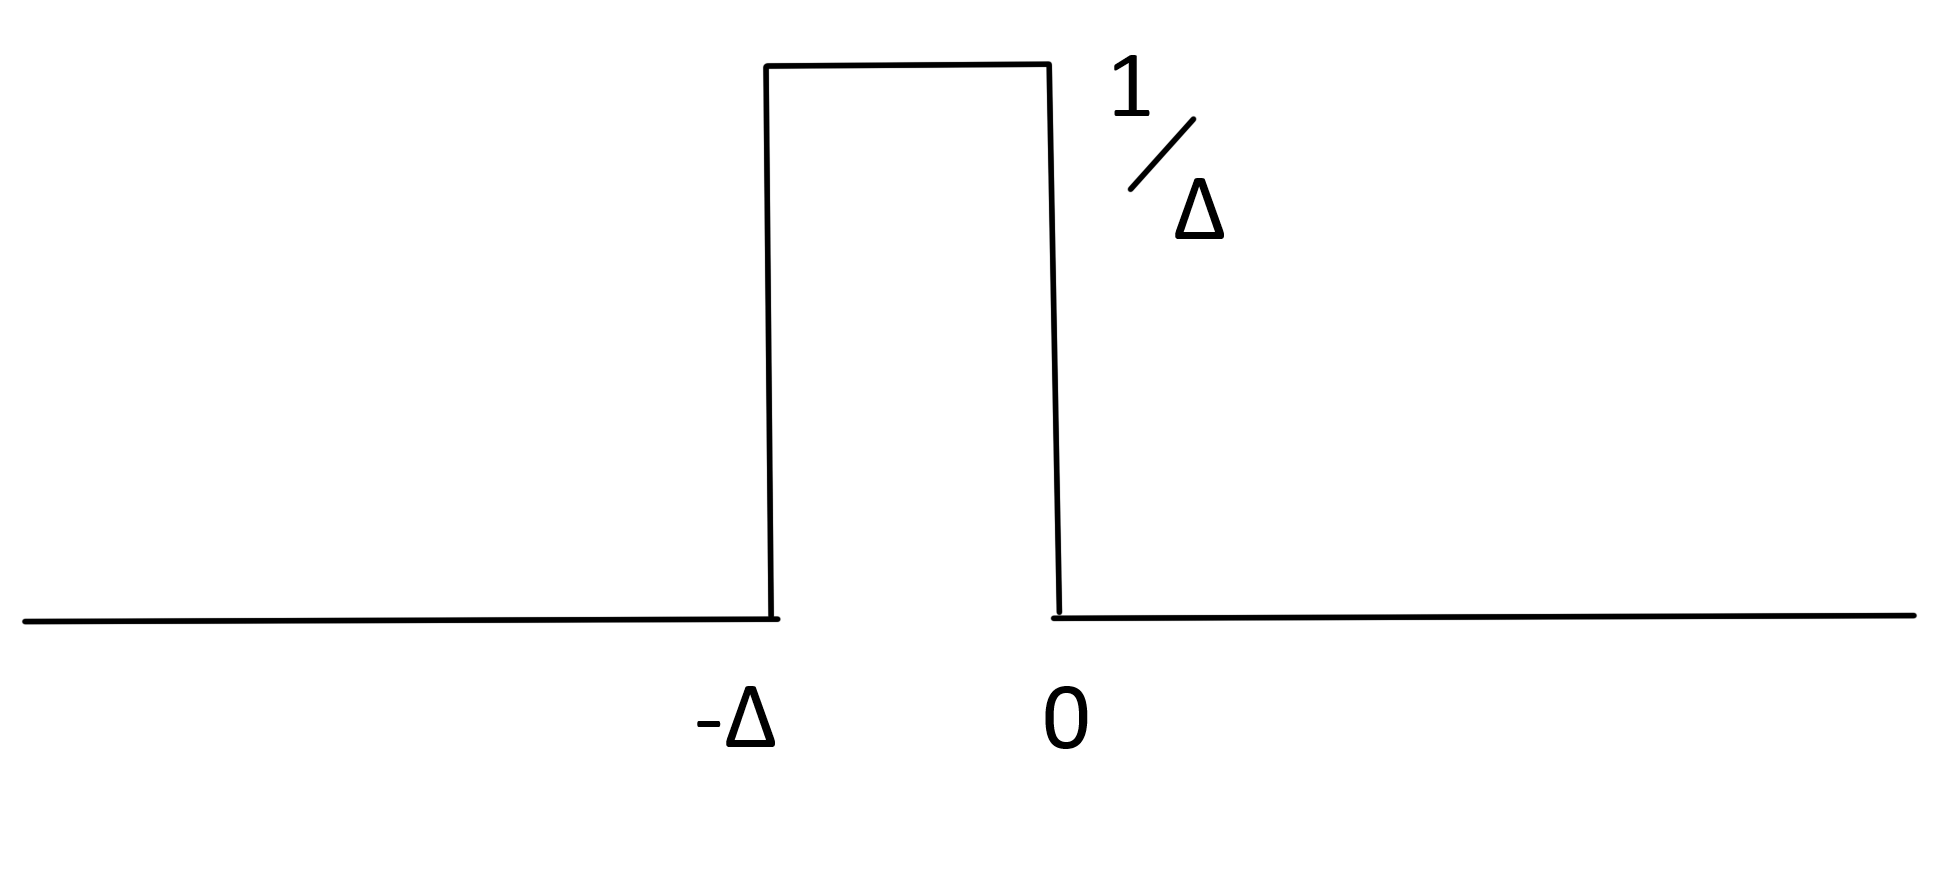
\includegraphics[width=0.6\textwidth]{./difference_deltas2.png}
	\caption{Difference of $u(t)$ and $u(t+\Delta)$, divided by $\Delta$}
\end{figure}
\indent which is nothing but the $\delta_\Delta$ function which we talked about. Taking the limit $\Delta\rightarrow0$, we get the derivative of $u(t)$ on one side, and the unit impulse $\delta(t)$ on the other.
Thus, there is a relationship of integration and differentiation between the unit step function and the unit impulse function. We have also found out the unit step response of the RC circuit. Since the derivative of the unit step function is the unit impulse function, is it true that the derivative of the unit step response for the RC circuit will give the unit impulse response?
More generally, if an input $x(t)$ produces an output $y(t)$ for an LSI system, does the derivative of $x(t)$ produce as the output, the derivative of $y(t)$?\\
\indent Intuitively, it seems to be correct, and taking the derivative of the unit step response for the RC circuit should give its unit impulse response. This question will be answered in the next lecture.
